\section{Metodika porovnávání \CICD systémů}
    U každého systému se nejprve seznámím s aktuální dokumentací. \CICD systémy provozované pouze jako \glstext{SaaS} (\textit{Software as a Service}) budu muset testovat v cloudu. Pokud systém nabízí self-hosted variantu, zprovozním ji na lokálním virtuálním serveru. Pro systémy s oficiálním kontejnerem budu systém spouštět v Dockeru. V případě, že systém má několik oficiálních variant instalace a nabízí jinou funkcionalitu (to je případ GitLabu), nainstaluji a otestuji systém několikrát. Všechny instalace budou nascriptované a opakovatelné. Technickou část práce netýkající se přímo daných \CICD systémů popisuji \pfxref{v příloze}{ch:implementace}.

    Na instalovaných systémech pak provedu základní nezbytné nastavení: to bude pravděpodobně konfigurace veřejné \glstext{URL}, případně portů. Dále bude nutná konfigurace vzdálené správy repozitářů, pokud ho \CICD nástroj nemá přímo zabudovaný. Bez dalšího nastavení zhodnotím zvlášť aplikační dostupnost za provozu a za správcovských úkonů: samostatně pro pro aktualizace \CI systému a pro rekonfiguraci. Tím se dozvím, jestli se lze spolehnout na výchozí nastavení dodavatele. Dostupnost budu měřit nástrojem \code{siege} \cite{fulmer-siege}. Jde o podobný nástroj jako je Apache \code{ab} \cite{apache-ab}, který navíc umí parsovat přijaté \glstext{HTML} a odesílat další požadavky na odkázané javascripty, kaskádové styly a další zdroje. Simuluje tak lépe chování uživatelů s webovým prohlížečem. Dostupnost budu testovat kontinuálními požadavky bez prodlev (volba \code{--benchmark}) s 10 uživateli (\code{--concurrent=10}). Výsledkem testu je počet selhaných požadavků, měřených podle \HTTP kódu odpovědi. Ideální výsledek je 0 selhaných požadavků. Dostupnost za klasického provozu aplikace budu měřit po dobu 15 minut. U administrátorských úkonů budu dostupnost měřit po celou dobu úkonu, která se bude lišit.

    Následně nakonfiguruji systém tak, aby měl co nejlepší možnou dostupnost a opět zopakuji testy na dostupnost.

    Na třech ukázkových projektech otestuji možnosti \CI, které systém nabízí. Aplikační testy budu z části simulovat jednoduchým bash scriptem.  Zaměřím se na: sledování stavu testů a přehlednost (logování, reporting), možnosti debugování (vzdálené připojení do testovacího prostředí, \code{ssh}), uchovávání artefaktů (výsledků kompilace), konfigurace v kódu (vs konfigurace klikáním v administraci).

    \subsection{P1: Jednoduchá aplikace bez externích závislostí}
        Tato kategorie pokrývá výhradně statické weby. Aplikace může obsahovat dynamické části jako je například kontaktní formulář, ale samotné zpracování se děje mimo statickou aplikaci -- cílem formulářů může být například Google Form \cite{mccoy-google-form}, nebo jiné aplikace (ať už třetích stran nebo vlastní).

        Pro testování \CICD systémů jsem vytvořil jednoduchý statický projekt s nástrojem Jekyll \cite{jekyll}. Ten ze zdrojových souborů které se skládají hlavně z Markdown textů \cite{markdown}, metadat a šablon generuje statické \HTML soubory. Dále umí kompilovat i styly, což jsem využil pro jednoduchý \code{scss} soubor. Na závěr každé kompilace se všechny assety přemístí do složky podle aktuálního data. Tím je aplikace připravena pro nasazení současně se starší nebo novější verzí.

        Při \CICD se typicky v repozitáři uchovávají pouze zdrojová data. Pro generátory statických webů to mohou být například soubory ve formátu Markdown a specifikace \HTML šablon. Z těch se pak v rámci buildu na \CICD pipeline vygenerují výsledné \HTML soubory. Je vhodné, aby statické zdroje (JavaScripty, kaskádové styly, \ldots) byly vygenerovány do unikátní složky, například podle verze buildu nebo podle času. Samotné nasazení na produkční server pak lze udělat bez výpadku tak, jak \pfxref{ilustruje diagram}{fig:static-deploy}: nejprve je nutné nasadit nové statické zdroje. Ty mají unikátní názvy (nejlépe jsou v unikátně pojmenovanné složce), takže jejich nasazení nepřepíše současné soubory. Následně se přepíší \HTML soubory. Uživatelé kteří ještě načetli starou verzi načtou staré zdroje. \HTML soubory neexistující v nové verzi lze po uvážení z produkčního serveru odstranit. Není potřeba invalidovat cache, protože nové zdroje jsou pojmenované jinak než ty staré. Po uplynutí vhodného času lze staré zdrojové soubory ze serveru smazat. Pro vysokou dostupnost je vhodné použít víc než jeden server. V tom případě stačí nahrát nové zdroje na všechny servery a po bariéře přepsat všechna \HTML.

        \begin{iffigure}
            \centering
            \makebox[\textwidth][c]{
                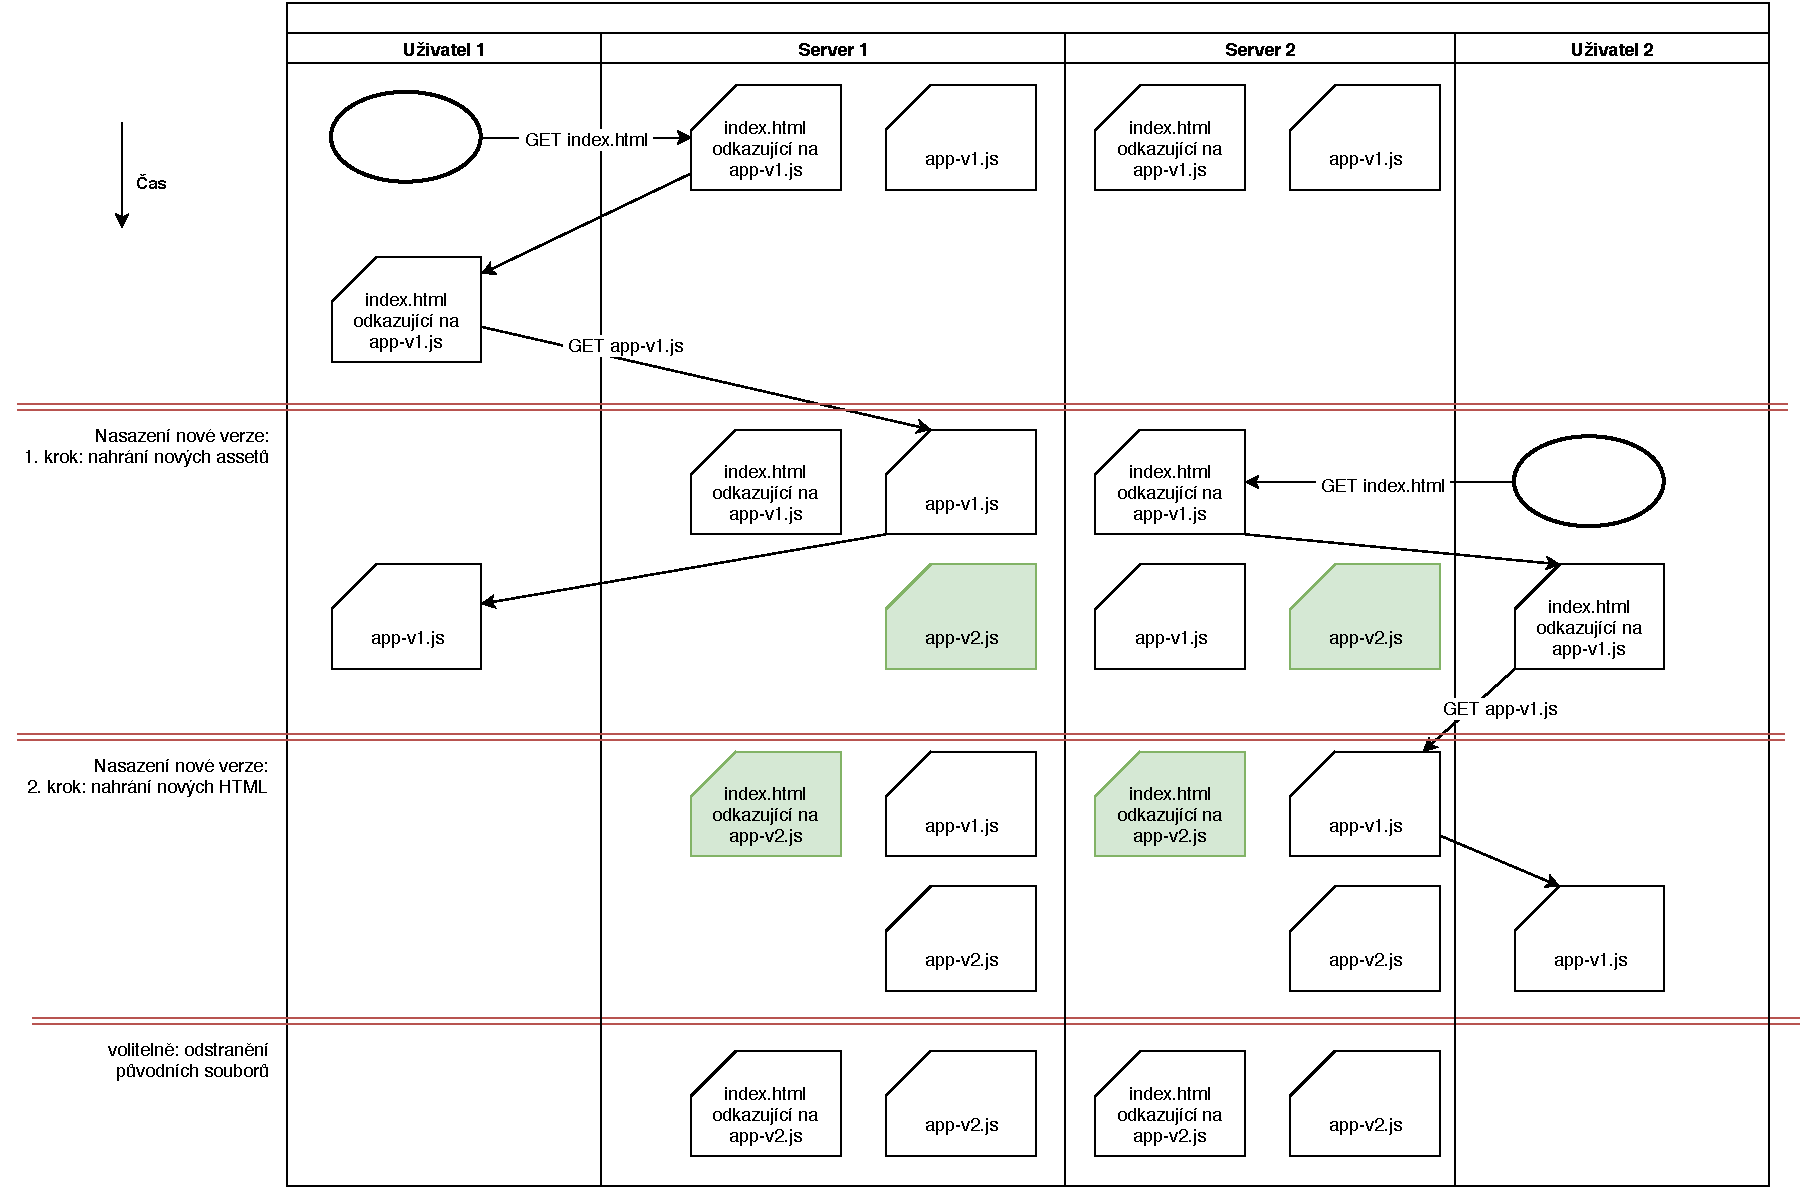
\includegraphics[width=1.2\textwidth]{media/static-deploy-changes.pdf}
            }
            \caption{Časový diagram znázorňující požadavky od dvou různých uživatelů ve dvou fázích nasazení nové verze statické aplikace. Uživatel 1 ilustruje nutnost nahrát nejprve na všechny servery sdílené assety. \HTML musíme nahrát až v druhé fázi, aby bylo garantované, že uživatelé co načtou novou verzi \HTML budou mít možnost ze všech serverů stáhnout odkazované zdroje. Uživatel 2 znázorňuje, proč je nutné uchovávat na serveru i starší verze zdrojů. Ty můžeme smazat až po nějaké delší době. Čas plyne odshora dolů, červené dvojité čáry reprezentují synchronizační bariéru.}
            \label{fig:static-deploy}
        \end{iffigure}

        Při použití kontejnerů nelze snadno dosáhnout toho, aby v containeru byly nové a současně staré zdroje. Místo toho se problém přesune na nějakou vyšší vrstvu, například ingress controller. Ten může podle \HTTP kódu odpovědi rozhodnout, jeslti se pokusí přeposlat požadavek na jiný kontejner. Pokud uživatel stáhne \HTML z nové verze aplikace, ale request na \glstext{CSS} přijde na starý container a vrátí kód \textit{404 Not Found}, může ingress controller GET požadavek přeposlat na nový kontejner, kde soubor existuje. Alternativou je použití session affinity, například pomocí cookies nebo \glstext{IP} adresy. Nebo lze mezi ingress controller a kontejnery umístit nějakou cachující \HTTP vrstvu (HAProxy, Varnish), která prakticky v základním nastavení načte a uloží do paměti zdroje z obou verzí. Je pouze nutné ošetřit, aby HTML ze starých kontejnerů nepřepsalo \HTML z kontejnerů nových, což může rozhodnout například podle hlavičky \code{Last-Modified-At}. Tento proces je vizualizován \pfxref{na diagramu}{fig:static-deploy-container}.

        \begin{iffigure}
            \centering
            \makebox[\textwidth][c]{
                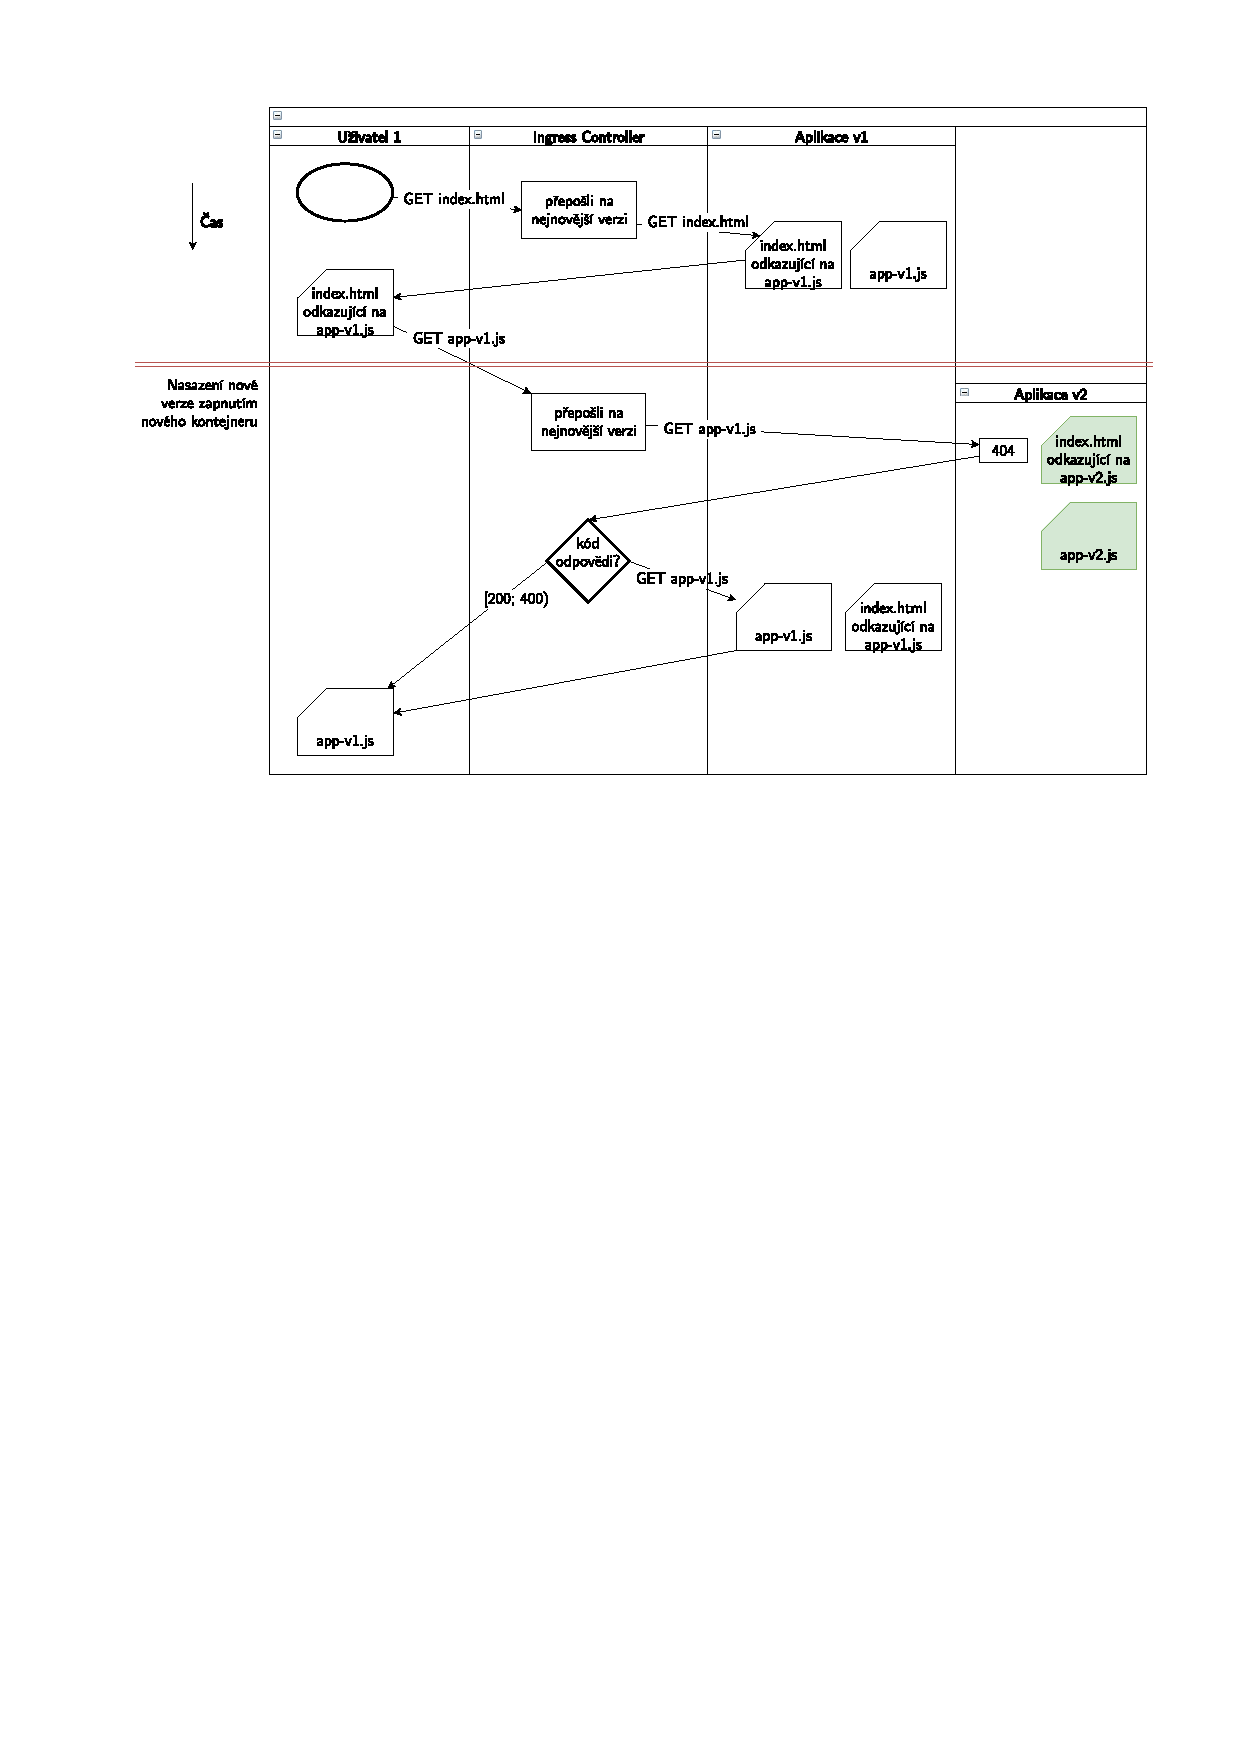
\includegraphics[width=1.2\textwidth]{media/static-deploy-kontejnery.pdf}
            }
            \caption{Časový diagram pro nasazení nové verze statické aplikace za použití kontejnerů. Pokud není praktické v nové verzi kontejneru uchovávat i starší verze zdrojů, je nutné implementovat nějakou komponentu (zde pojmenovanou \textit{ingress controller}), která při obdržení odpovědi s \glstext{HTTP} kódem 404 přepošle požadavek na starší verze aplikace. Toto chování je pro uživatele transparentní a projevuje se pouze lehce zvýšenou latencí.}
            \label{fig:static-deploy-container}
        \end{iffigure}

    \subsection{P2: Komplexní aplikace}
        V této kategorii uvažuji komplexní aplikace vyžadující relační databázi, případně další závislosti jako můžou být fronta, key-value storage, mailer, služba na zpracování obrázků nebo generování faktur, nebo platební brána. Na rozdíl od statických webů se tyto aplikace testují obtížně.
        U databáze například stačí spustit pro testy nový databázový stoj a spustit migrace. V případě platební brány která může od aplikace požadovat veřejně dostupnou url pro webhooks to může znamenat, že už samotný test vyžaduje nějakou úroveň nasazení aplikace.

        Pro testování jsem implementoval blog v PHP, konkrétně za použití frameworku Symfony \cite{symfony}. Aplikace při zpracování každého požadavku posílá dotazy na články do externí MySQL databáze. Dále komunikuje s key-value serverem Redis, kde spravuje session. Třetí závislost je API třetí strany: \code{mailgun.com}, které se používá pro posílání transakčních emailů.

    \subsection{P3: Aplikace distribuovaná jako kontejner}
        Aplikace v kontejneru mají stejné nároky na testovací prostředí jako aplikace v předchozí skupině a v rámci \CICD se liší pouze v buildu a nasazení. Jelikož samotné \CI často používá Docker, bude při tomto testu nutné řešit \glstext{DinD} nebo nějakou alternativu. Vystavěný Docker obraz je potřeba nahrát do nějakého repozitáře. Teoreticky lze obrazy exportovat/importovat i jako soubory, ale to není praktické, mj.~i proto, že se pak neuplatní sdílení jednotlivých vrstev obrazu. Některé systémy mají přímo zabudovaný registr obrazů a pro ostatní budu muset používat nějaký externí registr.
